
As an experiment toward future work, we tested the model on four zero-shot predictions on out-of-distribution, patient-specific aneurysm geometries. These new cases were selected from our internal database and exhibit a range of morphological variations, including aneurysm location, parent vessel diameter, neck size, aneurysm sac diameter, and centerline length. Their geometrical features are further described in \autoref{tab:0-shot_cases} and highlight the difference of these cases from the BenchAnXplore training and testing data. 

\begin{table}[!ht]
    \centering
    {\begin{tabular}{l c c c c c}
        \toprule
        \textbf{Case} & \small{\textbf{Location}} & \makecell{\small{\textbf{Inlet}}\\ \small{\textbf{diameter}}} & \makecell{\small{\textbf{Aneurysm}}\\ \small{\textbf{diameter}}} & \makecell{\small{\textbf{Aneurysm neck}}\\ \small{\textbf{diameter}}} & \makecell{\small{\textbf{Centerline}}\\ \small{\textbf{Length}}}\\
        \midrule \midrule
        \textbf{Case 1} & \text{ICA} & 4.8 & 4.5  & 4.2 & 49.1  \\
        \textbf{Case 2} & \text{MCA} & 2.5 & 6.0  & 5.2 & 23.2  \\
        \textbf{Case 3} & \text{MCA} & 2.7 & 7.8  & 7.3 & 21.4  \\
        \textbf{Case 4} & \text{ICA} & 4.3 & 15.0 & 8.7 & 65.5  \\
        \midrule \midrule
        \small{\textbf{BenchAnXplore}} & ICA & 4.0 & 3 - 9 & 3.2 & 25.6 \\
        \bottomrule
    \end{tabular}}
    \caption{Zero-shot cases geometrical description with aneurysm location, inlet artery diameter, aneurysm diameter, aneurysm neck diameter and artery centerline length from inlet to furthest outlet, all in mm. The BenchAnXplore values are given as a comparison.}
    \label{tab:0-shot_cases}
\end{table}

The In-PI-MGN model trained only on synthetic semi-idealized geometries was able to partially reproduce realistic flow behaviors in this complex clinical scenario. While the predicted velocity fields show discrepancies in order-of-magnitude for cases 3 and 4, the predicted velocity fields match the CFD ground truth in spatial distribution in all cases as shown in \autoref{fig:real_cases}. However, the model showed uneven behavior between cases, and while the predictions on these 4 cases are interesting, predictions on other cases were not as satisfying.

As highlighted by the promising yet degraded performance of our model on these out-of-distribution patient-specific cases (e.g., average 50-step relative velocity error on the four cases of 11\% compared to 1.6\% on the original test set), generalization to clinical settings requires training on representative data. 

\begin{figure}[!ht]
\centering
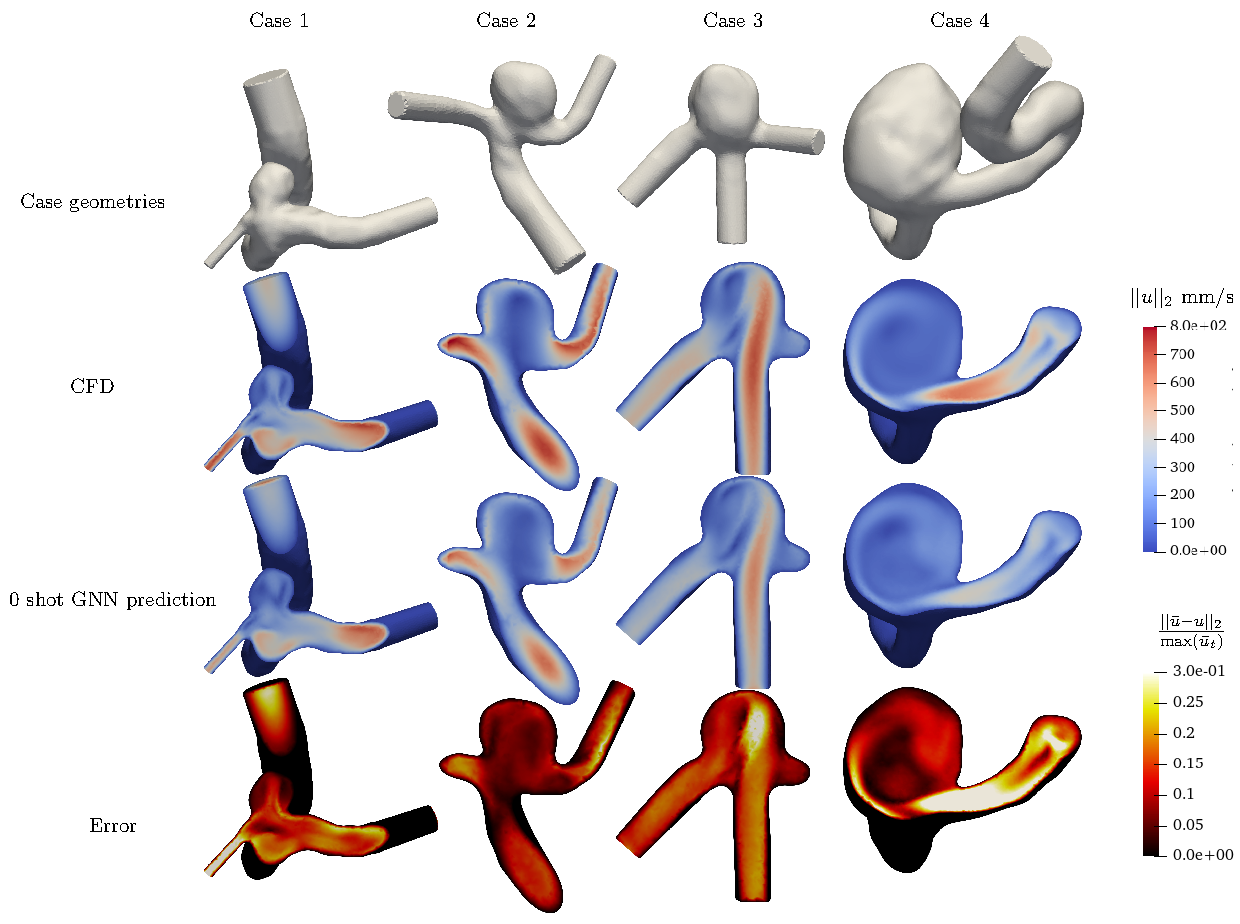
\includegraphics[width=1\textwidth]{figs/0shot_preds.pdf}
\caption{Zero-shot predictions on out-of-distribution patient-specific ICA and MCA aneurysm cases.}
\label{fig:real_cases}
\end{figure}

Building on this foundation, our following effort has been to build a more complex database to aim towards patient-specific robust hemodynamics. In the next chapter, we will try to address the limitations of the current work by working with more complex aneurysl cases as well as CFD-grade meshes and accurate WSS fields.
